\section{Gameplay Block Design}
\label{sec:game}

The gameplay module models the physics of the game, as well as outputs video
information to be displayed on screen. Based on information from the grab
button, player hand position, and
hcount and vcount signals, it determines which of the player's hands are
grabbing holds, and simulate their movement accordingly. Additionally, it is
able to provide a feedback signal to the glove module to signal when a players
hand is above a hold, and is not grabbing. The gameplay module is broken up into
four submodules: hand-holds, grabbing, movement, and pixel information, which
can be seen in figure \ref{fig:gameplay}. The hand-holds module keeps track of where the
hand holds are on the game map, and which onscreen pixels are occupied by hand
holds. The grabbing module takes this information, in addition to the player
hands positions from the tracking module, and grab information from the glove
module, and decides whether the player is grabbing onto any of the holds. The
movement module uses this grabbing information, and the players hand positions,
to simulate movement of the player. Finally, the pixel information module takes
the pixel by pixel information from the hand holds, as well as of the positions
of the players hands, and outputs pixel by pixel information, as well as its
corresponding hcount and vcount signals, to the VGA out component of the labkit.

Initially when integrating all parts of the gameplay module, clocking issues
were discovered, which resulted in incorrect colors, and minor artifacting. To
solve this problem, the clock, and all other signals, were pipelined throughout
the design. Information was passed linearly from hand-hold, to grab, to
movement, and finally to the pixel information module, instead of going straight
from the handhold to pixel information module, for example. Additionally, if one
stage took more than a single clock cycle to complete, its pipeline information
was delayed as well. This ensured proper syncing between all modules in the
gameplay block. The largest initial source of error in the design of the
gameplay module was mislabelled registers and wires. If there was even an error
in movement, it was almost always caused by either not declaring a register as
signed or indicating an incorrect number of bits. Both of which would lead to
sporadic movements. A photo of the game being played can be seen in figure
\ref{fig:playing}.

\begin{figure}[h]
\centering
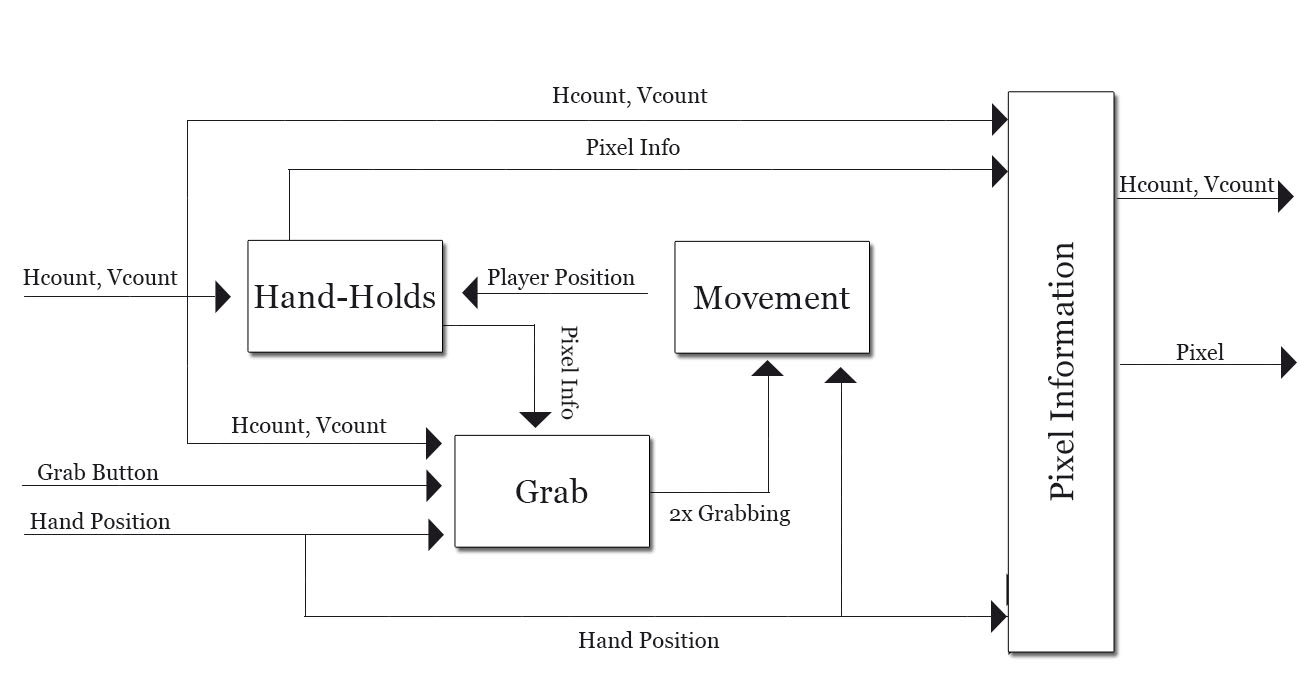
\includegraphics[width=6.5in]{img/gameplay.png}
\caption{The gameplay block is comprised of four modules: hand-holds, grabbing, movement, and pixel information}
\label{fig:gameplay}
\end{figure}

\begin{figure}[h]
\centering
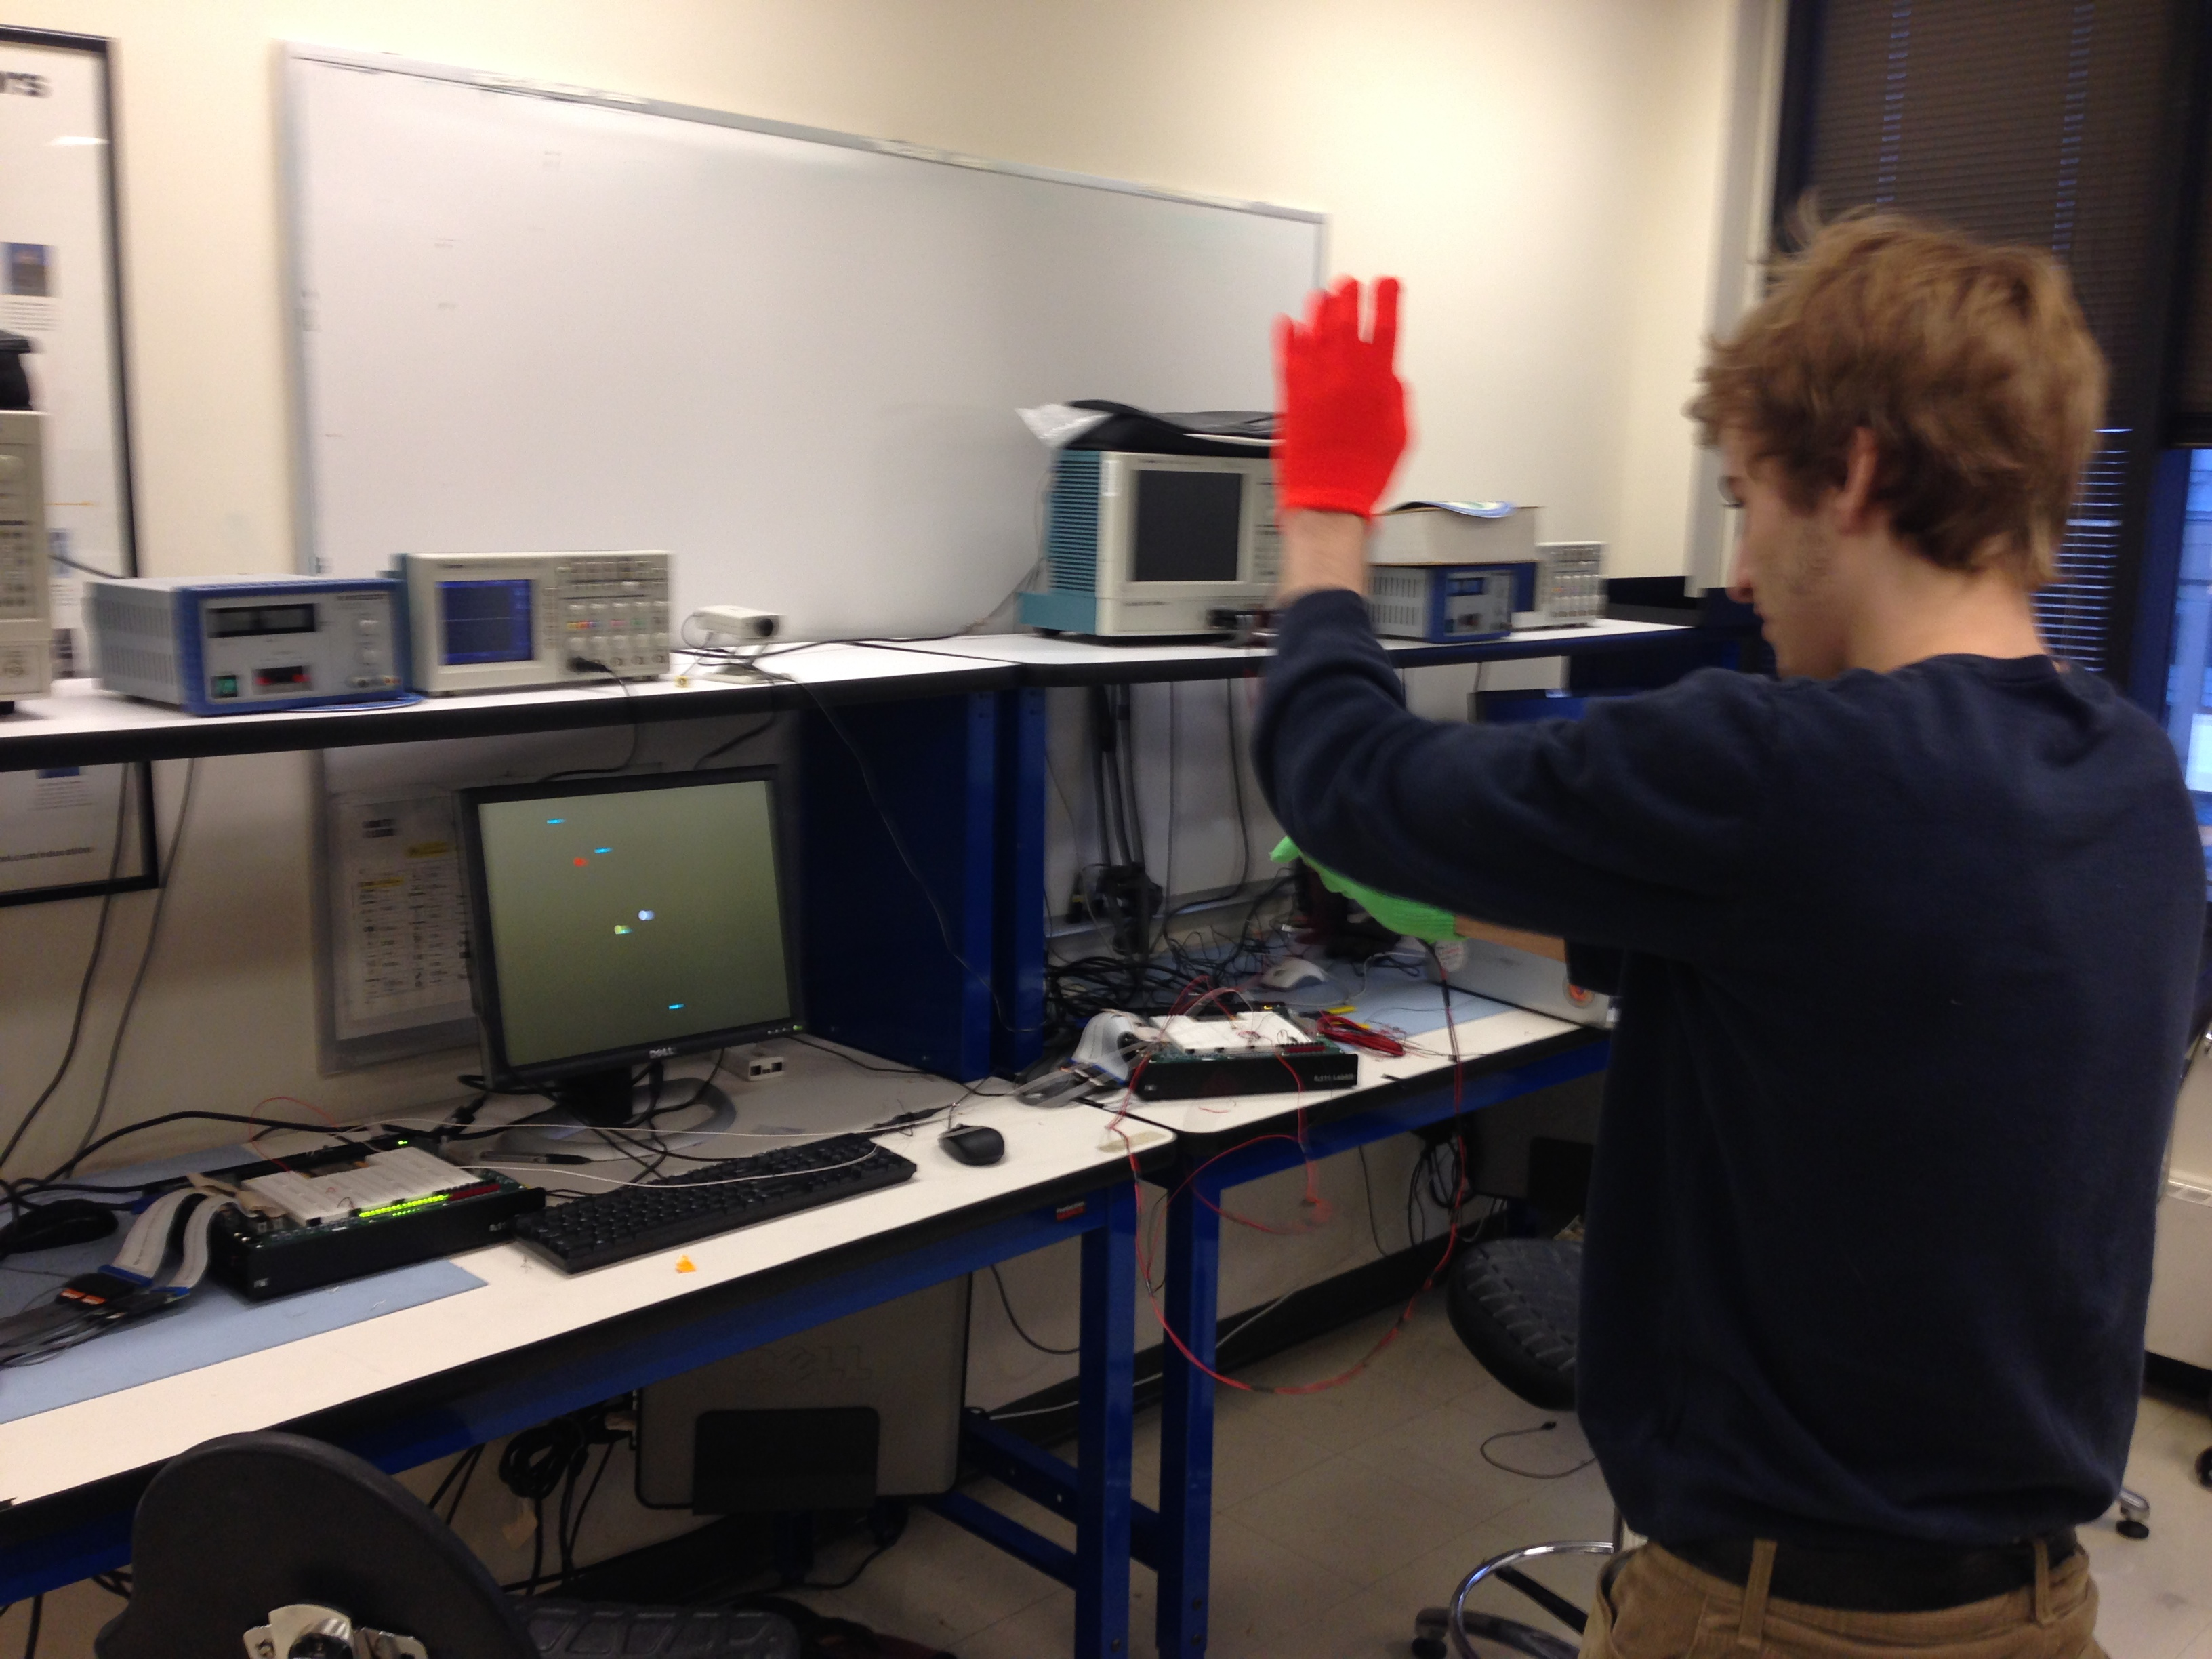
\includegraphics[width=6.5in]{img/playing.png}
\caption{A user plays the game by standing a short distance from the camera and
controlling their motion using their gloved hands.}
\label{fig:playing}
\end{figure}

\subsection{Hand-Holds}

The hand-hold submodule are in fact multiple submodules, however they act as
one. Each instance of the hand-hold module represents a single hold in the map,
and has an x and y coordinate associated with it, indicating its absolute
position. The holds have a width and a length, over which the holds are present.
Each hold sub-module takes in an hcount and vcount signal, as well as the
screen's absolute position information and determine, pixel by pixel, whether a
hand hold is present. This is done by adding the screen x and y coordinates to
the hcount and vcount coordinates, and seeing if they lie within the width and
height of each modules x and y coordinates. If it does, it outputs a one,
associated with the corresponding hcount and vcount signal. If not it outputs a
zero. The outputs of all of the individual hand hold modules with then be anded
together to signal if the current pixel, is occupied by any hand hold. By
default, the placement of the hand holds are predetermined. However, a map
editor was partially completed. By flipping a switch, the player can enter this
editing state. While in this state, the position of the screen tracks the
players hands, and they can grab holds to move them to new locations. While the
ability to grab and move holds was implemented successfully, the ability to
navigate the map while in the editing mode was glitchy, leading to an overall
failure of the map editting mode. This was most likely caused by a mislabed
register, or perhaps an unwanted feedback loop in the design.


\subsection{Grabbing}

For each hand, a grabbing module determines whether or not the player is
currently grabbing onto a hand hold, updating its output at every vsync. It does
it in a similar, pixel by pixel, manner as done in the hand-hold module. Its
inputs are hcount and vcount, the pixel by pixel “exist” signal coming from the
holds, hand positions relative to the screen, and signals coming from both of
the grab buttons. It has one output registers, grab, for each of the two hands.
When hcount and vcount are equal to one of the relative hand positions, it
checks to see if the player is pressing the corresponding grab button and if
there is a hand hold at that pixel. If these are all true, then it signals the
next output true. Otherwise it is set false. This is then sent to the movement
module.

\subsection{Movement}

The movement module is in charge of determining the players absolute position.
It uses the player's relative hand positions, grab information coming from the
grab module, and his previous velocity to do so. In actuality, the players
position is always fixed in relation to the camera, and is always displayed as a
fixed-position circle onscreen, so the movement module actually updates the
screen position. The screen position is then fed back to the hand-hold modules
at every vsync.

The movement module has two different states: one for when the player is
currently grabbing a hold, and one for free-fall. If the player is grabbing a
hold, their position is determined by an anchoring hand. This is to avoid
complications due to the player grabbing holds with both hands, and moving them
in a way that violates the game. Typically, the anchoring hand is the hand that
the player most recently grabbed a hold with. However, if the player lets go
with the anchoring hand, the movement module assigns the other as the anchoring
hand. Whenever a hand becomes the anchoring hand, its current relative position
is stored, as is the absolute position of the screen. When a player is grabbing
a hand hold, the movement module updates the camera position based on how far
the anchoring hand has moved since it first anchored. It subtracts the current
relative hand position from its relative anchored position and adds it to the
stored absolute screen position. If a player moves his anchored hand down, the
screen also shifts down, allowing the player to reach a higher hand-hold with
his non-anchored hand. If the player is not grabbing any hand-hold, he is in
freefall, with a corresponding x and y velocity. When he first releases his
hand, the game-play module averages his most recent velocities in the x and y
directions, and set that to his freefall velocity. With each frame, the movement
module updates the camera position based on this velocity, and the y velocity
are decremented in order to simulate gravity. This allows the player to quickly
pull down and release his grip, propelling him high into the air in order to
grab a previously unreachable hold.

\subsection{Pixel Information}

The pixel information module outputs a 24 bit, RGB color, along with
appropriately pipelined hcount, vcount, and vsync information, to a VGA output.
It takes in hcount and vcount signals, pixel information from the hand-hold
module, and player hand position to determine the value of the current pixel
output. It first checks to see if the hcount and vcount signals are within a
small radius from each hand position. If so, it sets the pixel output to red or
green, signifying player hand position. Otherwise it checks to see if the hcount
and vcount signals are within a small radius from the center of the screen. If
so it sets the pixel output to white, signifying the players position.
Otherwise, it check to see if the pixel information from the hand-hold module is
true. If so, it sets the pixel output to blue, indicating a hand hold. If none
of these are true, it displays a gradient background. It does this by adding the
vcount value to the negative screen position (as higher screen position have
more negative value). This is the gradient multiplier of each background pixel.
It then multiplies the R, G, and B values of each pixel by this multiplier and
shifts it 11 registers to the right (because the multiplier can be at most $2
^{11}$). If $vcount - screeny$ is greater than $2^{11}$, it sets the multiplier to
$2^{11}$ to avoid overflow errors.
